% 1977 年江苏徐州市,徐州地区初试卷第 7 题：一边靠墙的矩形猪圈示意图（按源卷第 2 页布局）。
% 斜纹线表示原有墙面，砖墙砌矩形的左、下、右三面，上边落在墙线上。
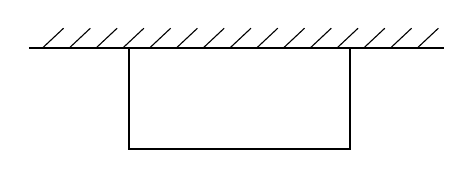
\begin{tikzpicture}[scale=0.85]
  \draw[thick] (-0.7,1.5) -- (5.5,1.5);
  \foreach \x in {-0.5,-0.1,...,5.1}
    \draw (\x,1.5) -- ++(0.32,0.3);
  \draw[thick] (0.8,1.5) -- (0.8,0) -- (4.1,0) -- (4.1,1.5);
\end{tikzpicture}
